\subsection{Kebutuhan \textit{Audit}}

Dalam merancang sebuah subsistem \textit{audit trail} yang andal, langkah pertama yang harus dilakukan adalah mengidentifikasi peristiwa (\textit{event}) apa saja yang esensial untuk direkam sebagai bukti digital. Penentuan kebutuhan \textit{audit event} ini tidak dilakukan secara acak, melainkan didasarkan pada pendekatan berbasis risiko. Oleh karena itu, analisis pada subbab ini diawali dengan mengevaluasi potensi ancaman keamanan pada arsitektur DecMed menggunakan pemodelan ancaman, yang hasilnya kemudian dipetakan menjadi daftar klasifikasi \textit{event} beserta atribut bukti yang dibutuhkan untuk keperluan mitigasi dan investigasi.

\subsection{Dekomposisi Aplikasi}

Dekomposisi aplikasi merupakan tahap awal proses \textit{threat modeling} yang bertujuan memperoleh pemahaman menyeluruh mengenai sistem DecMed dan bagaimana sistem tersebut berinteraksi dengan entitas eksternal. Dekomposisi ini terdiri atas deskripsi sistem, dependensi eksternal, titik masuk, aset, dan level kepercayaan, yang selanjutnya menjadi dasar bagi proses identifikasi ancaman menggunakan metode STRIDE.

\subsubsection{Deskripsi Sistem}

DecMed adalah kerangka kerja manajemen Rekam Medis Elektronik (RME) terdesentralisasi yang dibangun di atas Distributed Ledger Technology (DLT) IOTA. Sistem ini mengimplementasikan Capability-Based Access Control (CapBAC), Proxy Re-Encryption (PRE), dan InterPlanetary File System (IPFS) untuk menjamin kepemilikan data medis oleh pasien. Pasien secara aktif memberikan atau mencabut akses, menentukan durasi akses, dan berbagi data secara selektif dengan tenaga kesehatan. Sistem diimplementasikan menggunakan \textit{smart contract} berbahasa Move pada ledger IOTA, sementara data klinis terenkripsi disimpan pada IPFS.

Arsitektur sistem terdiri atas tiga lapisan (\textit{tiers}):
\begin{itemize}
    \item \textbf{Client Layer} -- antarmuka utama bagi seluruh aktor, dengan aplikasi \textit{client} yang disesuaikan per peran (mobile untuk pasien, desktop untuk tenaga fasyankes dan Kementerian Kesehatan), dibangun menggunakan \textit{framework} Tauri (Rust + SvelteKit/TypeScript).
    \item \textbf{Proxy Layer} -- middleware keamanan yang menegakkan kebijakan akses dan menangani operasi kriptografis (PRE), terdiri atas PRE Server (Rust, Axum) dan Gas Station Server.
    \item \textbf{Storage Layer} -- terbagi menjadi penyimpanan \textit{on-chain} (IOTA ledger, untuk metadata dan \textit{capability} akses) dan \textit{off-chain} (IPFS untuk data klinis terenkripsi, Redis untuk data sementara seperti \textit{nonce} dan \textit{kfrag}).
\end{itemize}

Seluruh akses terhadap data RME pasien oleh pihak lain wajib melalui Proxy, dan setiap pemberian akses oleh pasien dicatat sebagai entri \textit{capability} pada penyimpanan \textit{on-chain} yang bersifat \textit{immutable}, membentuk fondasi model CapBAC pada sistem DecMed.

\subsubsection{Dependensi Eksternal}

Dependensi eksternal merupakan objek di luar kode aplikasi yang keberadaannya dapat menimbulkan ancaman terhadap sistem. Setiap dependensi diberi nomor unik dan deskripsi.

\begin{xltabular}{\textwidth}{|>{\centering\arraybackslash}p{1.2cm}|>{\raggedright\arraybackslash}p{4.5cm}|X|}
    \caption{Dependensi Eksternal Sistem DecMed}
    \label{tab:dependensi-eksternal} \\
    \hline
    \textbf{ID} & \textbf{Komponen} & \textbf{Deskripsi} \\
    \hline
    \endfirsthead
    
    \hline
    \textbf{ID} & \textbf{Komponen} & \textbf{Deskripsi} \\
    \hline
    \endhead
    
    \hline
    \endfoot
    
    \hline
    \endlastfoot

    DE-01 & IOTA Rebased & DLT berbasis Directed Acyclic Graph (DAG) dengan konsensus Mysticeti (Byzantine Fault Tolerant, Delegated Proof-of-Stake), finalitas transaksi $\sim$500 ms, mendukung lebih dari 50.000 TPS. \\
    \hline

    DE-02 & Smart Contract Move & \textit{package} \texttt{decmed} yang dipublikasikan pada IOTA Layer 1, terdiri atas modul \texttt{patient}, \texttt{admin}, \texttt{hospital\_personnel}, \texttt{proxy}, \texttt{shared}, serta modul struktur data \texttt{std\_struct\_*} dan \texttt{std\_enum\_*}. \\
    \hline

    DE-03 & PRE Server & diimplementasikan dengan Rust dan \textit{framework} Axum, menyediakan endpoint REST untuk proses autentikasi, pertukaran kunci, dan operasi RME. \\
    \hline

    DE-04 & IOTA Gas Station & terdiri atas Gas Station Server (endpoint reservasi dan eksekusi \textit{gas object}), Gas Station Storage (berbasis Redis dengan skrip LUA untuk akses konkuren), dan Key Store Manager/KSM (KMS eksternal atau penyimpanan kunci \textit{in-memory}). \\
    \hline

    DE-05 & Redis & digunakan oleh PRE Server untuk menyimpan data sementara seperti \textit{nonce} autentikasi (TTL 3 menit) dan material PRE seperti \textit{kfrag} (TTL 2 jam); juga digunakan oleh Gas Station sebagai \textit{storage} \textit{gas object}. \\
    \hline

    DE-06 & IPFS Cluster & penyimpanan \textit{off-chain} terdesentralisasi berbasis \textit{content-addressing} (CID) untuk data klinis pasien yang telah dienkripsi, digunakan karena ukuran data klinis dapat melebihi batas objek IOTA (250 KB). \\
    \hline

    DE-07 & Client Application Framework & Tauri (Rust + SvelteKit/TypeScript), dengan tiga varian: Patient Client (mobile), Hospital Client (desktop), dan Ministry Client (desktop). \\
    \hline

    DE-08 & Skema BIP39 & standar \textit{mnemonic} 12 kata untuk pembuatan dan pemulihan kunci kriptografis pasien dan tenaga fasyankes secara \textit{non-custodial}. \\
    \hline

    DE-09 & Mekanisme kriptografis Proxy Re-Encryption (PRE) dan AES-GCM & digunakan untuk enkripsi data administratif dan klinis serta proses re-enkripsi \textit{ciphertext} bagi penerima yang berwenang. \\
    \hline

\end{xltabular}

\subsubsection{Titik Masuk}

Titik masuk (\textit{Entrypoints}) merupakan antarmuka pada aplikasi yang menjadi media interaksi antara pengguna (atau penyerang) dengan aplikasi maupun data. Setiap titik masuk diberi nomor unik, deskripsi, dan level kepercayaan minimum yang mengacu pada Tabel~\ref{tab:trust-level}.

\begin{xltabular}{\textwidth}{|>{\centering\arraybackslash}p{1.4cm}|>{\raggedright\arraybackslash}p{4.2cm}|X|>{\centering\arraybackslash}p{2cm}|}
    \caption{Titik Masuk Sistem DecMed}
    \label{tab:titik-masuk} \\
    \hline
    \textbf{ID} & \textbf{Nama} & \textbf{Deskripsi} & \textbf{Level Kepercayaan} \\
    \hline
    \endfirsthead
    \hline
    \textbf{ID} & \textbf{Nama} & \textbf{Deskripsi} & \textbf{Level Kepercayaan} \\
    \hline
    \endhead
    \hline
    \endfoot
    \hline
    \endlastfoot

    TM-01 & \texttt{POST /nonce} & Endpoint PRE Server untuk memperoleh \textit{nonce} autentikasi 64-byte, divalidasi melalui \textit{Move call} \texttt{is\_account\_registered}. & LK1--LK2 \\
    \hline

    TM-02 & \texttt{POST /keys} & Endpoint PRE Server untuk menyimpan material PRE (\textit{kfrag}, kunci publik) dan menerbitkan token akses JWT bagi tenaga fasyankes. & LK2 \\
    \hline

    TM-03 & \texttt{GET /medical-record} & Endpoint PRE Server untuk mengambil metadata administratif dan klinis pasien beserta proses re-enkripsi, memerlukan token akses \textit{read} yang valid. & LK4 \\
    \hline

    TM-04 & \texttt{POST /medical-record} & Endpoint PRE Server untuk membuat entri RME klinis baru, memerlukan token akses \textit{update}. & LK4 \\
    \hline

    TM-05 & \texttt{PUT /medical-record} & Endpoint PRE Server untuk mengubah entri RME klinis yang sudah ada pada kunjungan yang sama. & LK4 \\
    \hline

    TM-06 & \texttt{GET /medical-record/update} & Endpoint PRE Server untuk mengambil metadata RME sebelum proses pengubahan (edit). & LK4 \\
    \hline

    TM-07 & \texttt{GET /administrative} & Endpoint PRE Server untuk mengambil metadata administratif pasien, dapat diakses oleh admin fasyankes maupun tenaga administratif. & LK3, LK5 \\
    \hline

    TM-08 & Modul \texttt{decmed::patient} & Kumpulan \textit{method on-chain} yang dapat dieksekusi pasien: \texttt{signup}, \texttt{create\_access}, \texttt{revoke\_access}, \texttt{update\_administrative\_metadata}, \texttt{get\_medical\_record(s)}, \texttt{get\_access\_log}, dan sejenisnya. & LK1--LK2 \\
    \hline

    TM-09 & Modul \texttt{decmed::hospital\_personnel} & Kumpulan \textit{method on-chain} bagi tenaga fasyankes: \texttt{signup}, \texttt{use\_activation\_key}, \texttt{create\_activation\_key}, \texttt{cleanup\_read/update\_access}, \texttt{get\_read/update\_access}, dan sejenisnya. & LK3--LK5 \\
    \hline

    TM-10 & Modul \texttt{decmed::admin} & Kumpulan \textit{method on-chain} bagi Kementerian Kesehatan: \texttt{create\_activation\_key} (registrasi fasyankes), \texttt{update\_activation\_key}, \texttt{get\_hospitals}. & LK6 \\
    \hline

    TM-11 & Modul \texttt{decmed::proxy} & Kumpulan \textit{method on-chain} yang dieksekusi oleh PRE Server: \texttt{create\_capability}, \texttt{create/update\_medical\_record}, \texttt{get\_administrative\_data}, \texttt{get\_hospital\_personnel\_role}, dan sejenisnya. & LK7 \\
    \hline

    TM-12 & Gas Station endpoint (\textit{reserve} \& \textit{execute}) & Dua endpoint utama Gas Station Server untuk mencadangkan objek \textit{gas} dan mengeksekusi transaksi tersponsori atas nama \textit{client}. & LK7, LK8 \\
    \hline

    TM-13 & QR Code Delegasi Akses & Antarmuka fisik/visual berisi \texttt{iota\_address} dan \texttt{pre\_public\_key} tenaga medis, dipindai oleh Patient Client untuk memulai proses delegasi akses. & LK2, LK4 \\
    \hline

    TM-14 & Sign-in lokal (PIN/biometrik) & Mekanisme autentikasi harian pasien/tenaga fasyankes menggunakan PIN atau biometrik terhadap kunci privat yang tersimpan terenkripsi di perangkat. & LK1--LK5 \\
    \hline

\end{xltabular}

\subsubsection{Aset}

Aset merupakan hal fisik maupun abstrak yang dimiliki sistem dan menjadi target ketertarikan penyerang. Setiap aset diberi nomor unik, deskripsi, dan level kepercayaan yang mengacu pada Tabel~\ref{tab:trust-level}.

\begin{xltabular}{\textwidth}{|>{\centering\arraybackslash}p{1.2cm}|>{\raggedright\arraybackslash}p{3.5cm}|X|}
    \caption{Aset Sistem DecMed}
    \label{tab:aset} \\
    \hline
    \textbf{ID} & \textbf{Nama} & \textbf{Deskripsi} \\
    \hline
    \endfirsthead
    \hline
    \textbf{ID} & \textbf{Nama} & \textbf{Deskripsi} \\
    \hline
    \endhead
    \hline
    \endfoot
    \hline
    \endlastfoot

    A-01 & Data administratif RME & Identitas dan data sosial pasien (NIK, nama, dsb.), terenkripsi AES-GCM sebelum disimpan \textit{on-chain}. \\
    \hline

    A-02 & Data klinis RME & Data pemeriksaan, diagnosis, dan tindakan medis, terenkripsi AES-GCM dan disimpan pada IPFS sebagai \texttt{enc\_medical\_data}. \\
    \hline

    A-03 & Entri \textit{capability} akses (\textit{on-chain}) & Struktur data \texttt{hospital\_personnel\_access\_data} berisi \texttt{access\_data\_types}, \texttt{exp} (durasi kedaluwarsa), \texttt{metadata}, dan \texttt{medical\_metadata\_index} -- fondasi model CapBAC. \\
    \hline

    A-04 & \textit{Recovery phrase} (BIP39) \& kunci privat pasien/personel & \textit{Mnemonic} 12 kata dan kunci privat turunannya, disimpan terenkripsi pada perangkat menggunakan \textit{secure hardware}. \\
    \hline

    A-05 & Material PRE (\texttt{kfrag}, \texttt{cfrag}, \textit{pre\_secret/public\_key}) & Komponen kriptografis yang memungkinkan proses re-enkripsi data pasien kepada penerima yang berwenang. \\
    \hline

    A-06 & \textit{Nonce} autentikasi & Nilai acak 64-byte, TTL 3 menit, disimpan di Redis untuk mencegah serangan \textit{replay} pada proses autentikasi pasien. \\
    \hline

    A-07 & Token akses JWT & Token dengan klaim \textit{role} dan \textit{access type} (Read/Update); durasi berbeda antara tenaga medis (15 menit baca, 2 jam tulis) dan tenaga administratif. \\
    \hline

    A-08 & \textit{Activation key} & Kredensial sekali pakai yang diterbitkan Kementerian Kesehatan (untuk admin fasyankes) dan admin fasyankes (untuk personel), berfungsi sebagai \textit{cryptographic witness} atas tindakan yang diotorisasi. \\
    \hline

    A-09 & \texttt{GlobalAdminCap} \& \texttt{ProxyCapEnum} & Representasi \textit{capability} tertinggi pada sistem -- masing-masing untuk Kementerian Kesehatan dan PRE Server; kompromi terhadap aset ini setara dengan eskalasi privilese total. \\
    \hline

    A-10 & CID data klinis (IPFS) & \textit{Content Identifier} yang menjadi referensi lokasi dan \textit{fingerprint} integritas data klinis terenkripsi pada IPFS. \\
    \hline

    A-11 & \textit{Gas object} \& kunci penandatanganan Gas Station & Token IOTA yang dipecah menjadi objek \textit{gas} untuk mensponsori transaksi, beserta kunci penandatanganan yang dikelola KSM. \\
    \hline

    A-12 & Log akses RME & Catatan riwayat akses terhadap data RME pasien, dapat dilihat pasien melalui \texttt{get\_access\_log}. \\
    \hline

\end{xltabular}

\subsubsection{Level Kepercayaan}

Level kepercayaan merepresentasikan hak akses yang diberikan sistem kepada suatu entitas eksternal maupun proses internal. Penentuan level kepercayaan pada sistem DecMed menggunakan pendekatan gabungan (\textit{hybrid}) antara \textit{role} untuk entitas eksternal (manusia) dan \textit{capability} untuk proses/entitas internal, mengingat sistem DecMed secara eksplisit mengimplementasikan model Capability-Based Access Control (CapBAC).

\begin{xltabular}{\textwidth}{|>{\centering\arraybackslash}p{1.2cm}|>{\raggedright\arraybackslash}p{3.3cm}|X|}
    \caption{Level Kepercayaan Sistem DecMed}
    \label{tab:trust-level} \\
    \hline
    \textbf{ID} & \textbf{Nama} & \textbf{Deskripsi} \\
    \hline
    \endfirsthead
    \hline
    \textbf{ID} & \textbf{Nama} & \textbf{Deskripsi} \\
    \hline
    \endhead
    \hline
    \endfoot
    \hline
    \endlastfoot

    LK1 & Aktor belum teraktivasi/teregistrasi & Pengguna yang belum menyelesaikan proses \textit{signup} atau aktivasi \textit{client}; tidak memiliki \textit{capability} apa pun pada sistem. \\
    \hline

    LK2 & Pasien (teraktivasi) & Pasien yang telah teregistrasi; memiliki \textit{capability} membaca RME sendiri, memberi dan mencabut akses, serta melihat log akses. \\
    \hline

    LK3 & Administrative Personnel (dengan \textit{capability} aktif) & Tenaga administratif fasyankes yang telah diberi akses oleh pasien; \textit{scope} akses terbatas pada data administratif saja. \\
    \hline

    LK4 & Medical Personnel (dengan \textit{capability} aktif) & Tenaga medis fasyankes yang telah diberi akses oleh pasien; \textit{scope} akses mencakup data administratif dan klinis, termasuk hak tulis (tambah/ubah) data klinis. \\
    \hline

    LK5 & Hospital Admin & Administrator fasyankes; berwenang menambah personel dan menerbitkan \textit{activation key} pada lingkup fasyankesnya. \\
    \hline

    LK6 & Ministry of Health & Administrator Kementerian Kesehatan; berwenang meregistrasi fasyankes baru beserta admin-nya, otoritas tertinggi di antara aktor manusia. \\
    \hline

    LK7 & PRE Server (Proxy) & Proses \textit{backend} dengan \textit{capability} \texttt{ProxyCapEnum}; berwenang memverifikasi entri \textit{capability on-chain} dan melakukan re-enkripsi data. \\
    \hline

    LK8 & Gas Station Server & Proses \textit{backend} yang mensponsori dan mengeksekusi transaksi atas nama \textit{client}, memiliki akses terhadap kunci penandatanganan (KSM). \\
    \hline

    LK9 & IOTA Network Validator & Node jaringan yang berpartisipasi dalam konsensus Mysticeti untuk memvalidasi dan memfinalisasi transaksi pada ledger IOTA. \\
    \hline

\end{xltabular}

Catatan: LK3 dan LK4 bersifat \textit{paralel}, bukan hierarkis -- keduanya diberikan \textit{capability} oleh pasien secara independen dengan cakupan data yang berbeda (administratif saja vs. administratif dan klinis), sehingga tidak dapat diasumsikan LK4 selalu memiliki privilese lebih tinggi dari LK3 di seluruh konteks ancaman.

\subsubsection{Data Flow Diagram}

Data Flow Diagram (DFD) digunakan untuk menggambarkan aliran data antara entitas eksternal, proses, dan penyimpanan data pada sistem DecMed secara visual, sebagai dasar identifikasi elemen yang akan diklasifikasikan ancamannya menggunakan metode STRIDE pada subbab berikutnya. DFD sistem DecMed digambarkan pada Gambar~\ref{fig:decmed-dfd}.

\begin{figure}[h]
    \centering
    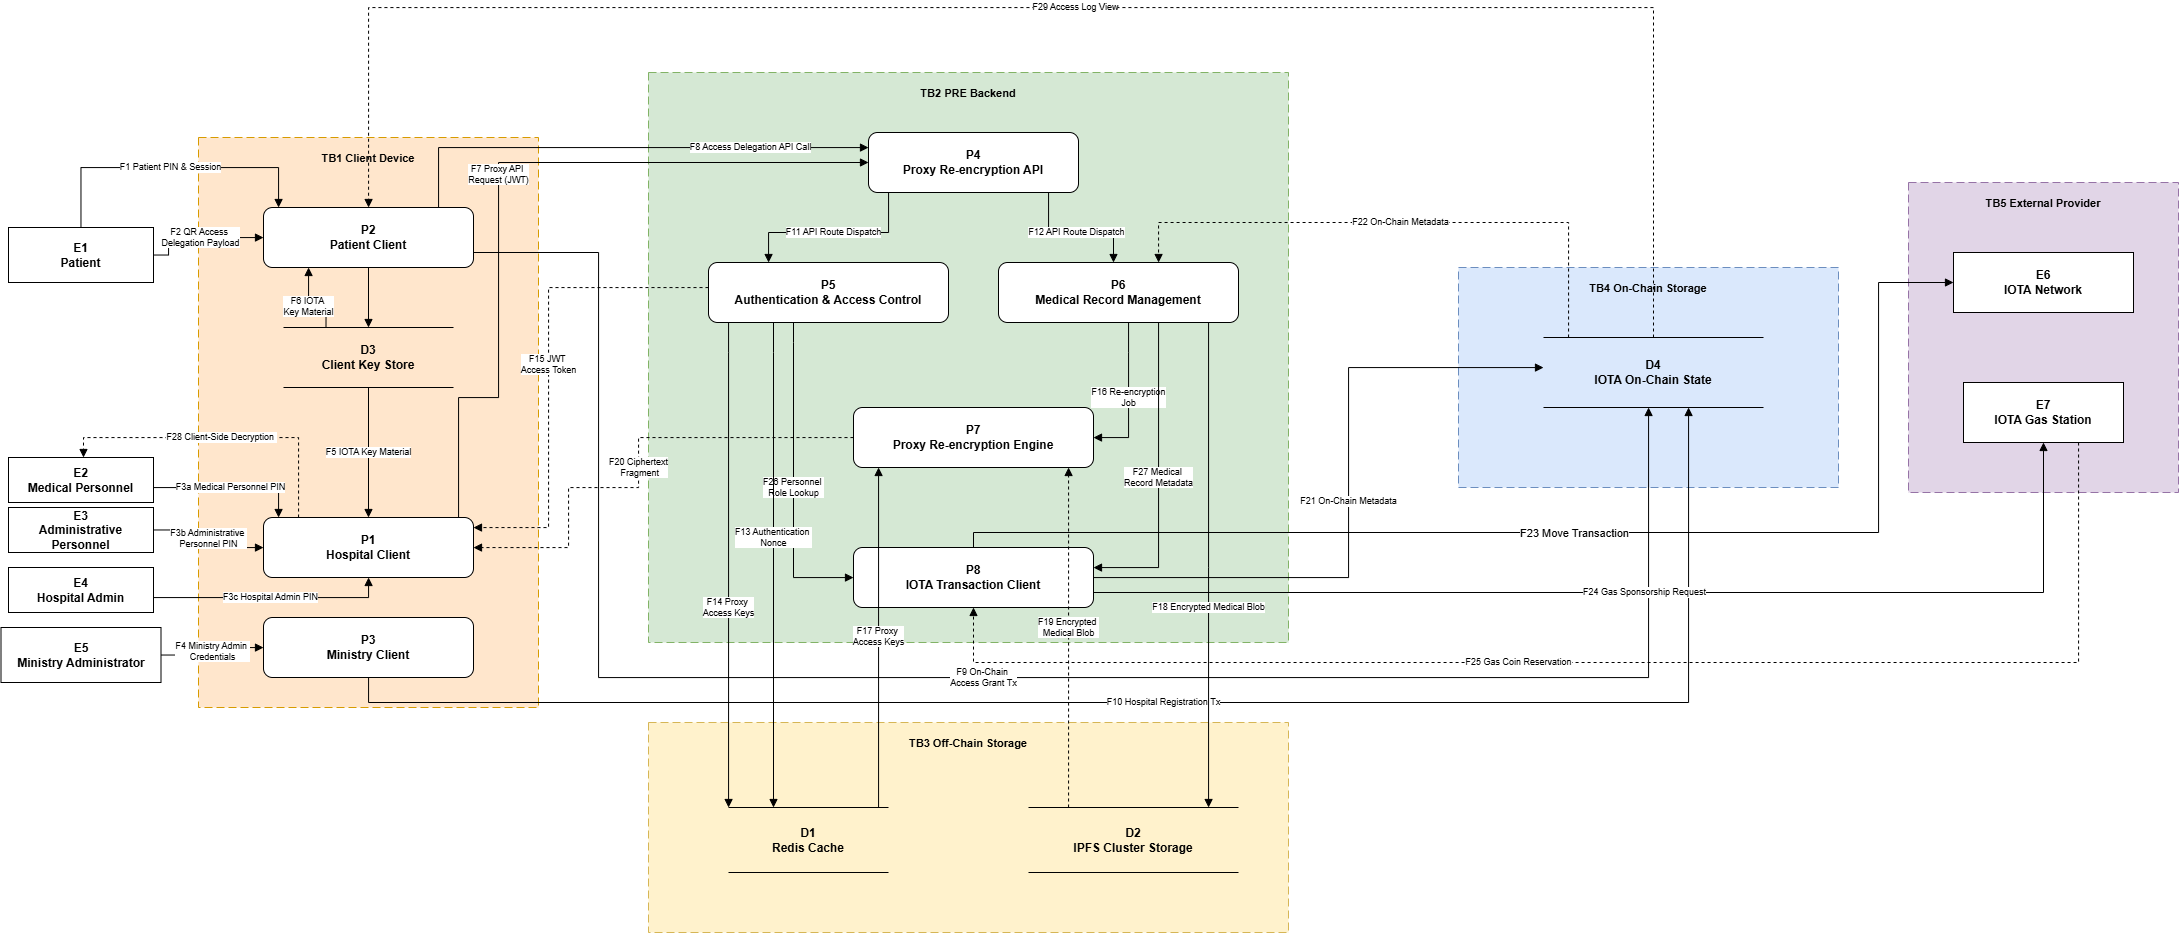
\includegraphics[width=\textwidth]{resources/chapter-3/final-decmed-dfd.png}
    \caption{Data Flow Diagram Sistem DecMed}
    \label{fig:decmed-dfd}
\end{figure}

DFD tersebut menggambarkan interaksi antara entitas eksternal (aktor), proses, dan penyimpanan data yang telah diidentifikasi pada dependensi eksternal (Tabel~\ref{tab:dependensi-eksternal}), titik masuk (Tabel~\ref{tab:titik-masuk}), aset (Tabel~\ref{tab:aset}), dan level kepercayaan (Tabel~\ref{tab:trust-level}) pada subbab sebelumnya. Elemen-elemen pada DFD tersebut menjadi dasar penomoran dan referensi pada proses identifikasi ancaman menggunakan metode STRIDE (III.1.2.2).

\subsection{Identifikasi Ancaman DecMed}

Identifikasi ancaman dilakukan menggunakan pendekatan \textit{STRIDE-per-Interaction}. Setiap interaksi antar elemen pada Data Flow Diagram (Gambar~\ref{fig:decmed-dfd}) diperiksa berdasarkan arah dan tipe interaksinya (\textit{process} ke \textit{data store}, \textit{process} ke \textit{process}, \textit{data flow} yang melintasi \textit{machine boundary}, dsb.), kemudian kategori STRIDE yang dianalisis dibatasi hanya pada kategori yang relevan bagi tipe interaksi tersebut, mengacu pada Tabel~\ref{tab:stride-per-interaction}. Pendekatan ini memberikan justifikasi eksplisit atas kategori yang dipilih maupun yang tidak dianalisis untuk setiap ancaman.

Elemen \texttt{E6 IOTA Network} dan \texttt{E7 IOTA Gas Station} pada \texttt{TB5 External Provider} diperlakukan sebagai infrastruktur eksternal tepercaya yang berada di luar kendali sistem DecMed; ancaman terhadap operasional internal keduanya berada di luar cakupan \textit{threat model} ini, dan hanya interaksinya dengan sistem (melalui P8, sebagai \textit{process} yang mengirim output ke \textit{external interactor}) yang dianalisis.

Hasil identifikasi ancaman disajikan pada Tabel~\ref{tab:klasifikasi-ancaman}, dengan kolom \textbf{Tipe Interaksi} merujuk pada nomor baris interaksi di Tabel~\ref{tab:stride-per-interaction} yang menjadi dasar penentuan kategori STRIDE bagi ancaman terkait.

\begin{xltabular}{\textwidth}{|>{\centering\arraybackslash}p{0.8cm}|X|>{\centering\arraybackslash}p{1.3cm}|>{\centering\arraybackslash}p{1.5cm}|>{\centering\arraybackslash}p{1.5cm}|>{\centering\arraybackslash}p{1.5cm}|}
    \caption{Identifikasi Ancaman Sistem DecMed} 
    \label{tab:klasifikasi-ancaman} \\
    
    \hline
    \textbf{ID} & \textbf{Deskripsi Ancaman} & \textbf{Elemen DFD} & \textbf{Level Kepercayaan} & \textbf{Tipe Interaksi} & \textbf{STRIDE} \\
    \hline
    \endfirsthead

    \hline
    \textbf{ID} & \textbf{Deskripsi Ancaman} & \textbf{Elemen DFD} & \textbf{Level Kepercayaan} & \textbf{Tipe Interaksi} & \textbf{STRIDE} \\
    \hline
    \endhead

    \hline
    \endfoot

    \hline
    \endlastfoot

    T1 & Penyerang mendapatkan kredensial atau membajak sesi lokal milik pengguna untuk berpura-pura menjadi pemilik identitas sah saat \textit{sign-in}. & E1--E5, P1, P2, P3 & LK1--LK6 & 7, 11 & S \\
    \hline

    T2 & Kredensial \textit{sign-in} (PIN) tersadap atau terekam melalui \textit{shoulder surfing}, \textit{keylogger}, atau malware pada perangkat saat dimasukkan ke Client. & E1--E5, P1, P2, P3 & LK1--LK6 & 7, 11 & I \\
    \hline

    T3 & Percobaan \textit{sign-in} berulang secara masif menghabiskan sumber daya Client (\textit{local resource exhaustion}). & E1--E5, P1, P2, P3 & LK1 & 7 & D \\
    \hline

    T4 & Payload QR Access Delegation dipalsukan sebelum dipindai oleh Patient Client. & P2, F2 & LK2, LK4 & 7 & S \\
    \hline

    T5 & Payload QR Access Delegation disadap sehingga informasi delegasi akses bocor kepada pihak tidak berwenang. & P2, F2 & LK2, LK4 & 7 & I \\
    \hline

    T6 & Pasien menyangkal pernah memberikan akses (\texttt{create\_access}) kepada tenaga medis tertentu. & E1, P2, P8 & LK2 & 11 & R \\
    \hline

    T7 & Tenaga medis atau tenaga administratif menyangkal pernah mengakses maupun mengubah data pasien tertentu. & E2, E3, P1, P6 & LK3, LK4 & 11 & R \\
    \hline

    T8 & Admin fasyankes menyangkal pernah menerbitkan \textit{activation key} kepada personel tertentu. & E4, P1 & LK5 & 11 & R \\
    \hline

    T9 & Ministry Administrator menyangkal pernah meregistrasi fasyankes tertentu beserta admin-nya. & E5, P3 & LK6 & 11 & R \\
    \hline

    T10 & Penyerang menyamar sebagai Proxy Re-encryption API (P4) yang sah (\textit{man-in-the-middle}) saat Client mengirim permintaan, karena flow melintasi batas perangkat (\textit{client}--\textit{backend}). & P1, P2, P4, F7, F8 & LK2--LK4 & 2, 8 & S \\
    \hline

    T11 & Penyerang menyadap komunikasi Client--PRE Server yang melintasi batas perangkat, mengungkap token JWT maupun data administratif. & P1, P2, P4, F7, F8, F15 & LK2--LK4 & 8 & I \\
    \hline

    T12 & Pihak eksternal membanjiri \textit{endpoint} \texttt{POST /nonce} atau \texttt{POST /keys} dengan permintaan palsu untuk menghabiskan sumber daya PRE Server. & P4, P5, F7, F8 & LK1 & 7 & D \\
    \hline

    T13 & Token JWT dipalsukan atau diputar ulang (\textit{replay}) pada permintaan dari Proxy Re-encryption API ke Medical Record Management. & P4, P6, F12 & LK3, LK4 & 2 & S \\
    \hline

    T14 & Penyadapan jalur \textit{dispatch} internal dari Proxy Re-encryption API ke Authentication/Medical Record Management mengungkap data yang sedang diproses. & P4, P5, P6, F11, F12 & LK7 & 2 & I \\
    \hline

    T15 & Penyerang memodifikasi \textit{Move transaction} pada jalur dari IOTA Transaction Client menuju IOTA Network, karena flow melintasi batas sistem DecMed dengan infrastruktur eksternal. & P8, F23 & LK7, LK8 & 3, 8 & T \\
    \hline

    T16 & Penyerang menyamar sebagai IOTA Transaction Client (P8) yang sah saat berinteraksi dengan Gas Station untuk mengajukan sponsorship transaksi palsu. & P8, F24 & LK7, LK8 & 3 & S \\
    \hline

    T17 & PRE Server (P8) menyangkal telah mengajukan atau menerima keputusan sponsorship transaksi tertentu dari Gas Station. & P8, F24, F25 & LK7, LK8 & 3 & R \\
    \hline

    T18 & Penyerang mengajukan permintaan sponsorship \textit{gas} secara berulang sehingga \textit{gas object} habis dan transaksi sah pengguna lain gagal tersponsori. & P8, F24, F25 & LK1--LK4 & 3 & D \\
    \hline

    T19 & Penyerang dengan akses tidak sah memodifikasi kunci privat atau material PRE yang tersimpan pada Client Key Store. & D3, P1, P2, F5, F6 & LK1 & 5, 10 & T \\
    \hline

    T20 & Penyerang dengan akses fisik ke perangkat yang tidak terkunci membaca kunci privat pada Client Key Store. & D3, F5, F6 & LK1 & 10 & I \\
    \hline

    T21 & Pihak dengan akses tidak sah ke Redis memodifikasi nilai \textit{nonce} autentikasi atau \texttt{kfrag} sebelum digunakan. & D1, P4, P5, P7, F13, F14 & LK7 & 5, 10 & T \\
    \hline

    T22 & Pihak dengan akses tidak sah ke Redis membaca \texttt{kfrag} atau \textit{nonce} sebelum masa berlakunya (TTL) berakhir. & D1 & LK7 & 10 & I \\
    \hline

    T23 & Redis dipenuhi (\textit{memory exhaustion}) melalui permintaan \textit{nonce} baru secara berulang sehingga proses autentikasi pengguna sah terganggu. & D1, F13 & LK1 & 5 & D \\
    \hline

    T24 & Data klinis terenkripsi diunduh dari IPFS Cluster Storage oleh pihak tidak berwenang; risiko pengungkapan tetap ada apabila kunci enkripsi terkait bocor atau lemah. & D2, F18, F19 & LK1, publik & 10 & I \\
    \hline

    T25 & IPFS Cluster dibanjiri permintaan \textit{fetch}/\textit{pin} berukuran besar sehingga mengganggu ketersediaan data klinis bagi pengguna sah. & D2 & publik & 5 & D \\
    \hline

    T26 & Metadata \textit{on-chain} yang tersimpan pada IOTA On-Chain State bersifat publik sehingga pola transaksi berpotensi dianalisis untuk mengungkap informasi tidak langsung mengenai pasien. & D4, F21, F22 & LK9, publik & 10 & I \\
    \hline

    T27 & Kelemahan validasi \textit{capability on-chain} memungkinkan pembacaan atau pembuatan \texttt{ProxyCapEnum}/\texttt{GlobalAdminCap} tanpa otorisasi sah, setara privilese tertinggi PRE Server/Kementerian Kesehatan. & P7, D4 & LK2/LK4 $\rightarrow$ LK6/LK7 & 5 & E \\
    \hline

    T28 & Kegagalan validasi otorisasi pada Authentication \& Access Control memungkinkan Medical Record Management memproses permintaan dengan \textit{scope} lebih tinggi dari yang seharusnya (administratif $\rightarrow$ klinis). & P5, P6, F26 & LK3 $\rightarrow$ LK4 & 2 & E \\
    \hline

\end{xltabular}


\subsection{Analisis Kebutuhan Audit Event}

Berdasarkan hasil analisis ancaman menggunakan metode STRIDE pada bagian sebelumnya, tahap selanjutnya adalah menentukan kebutuhan audit trail yang diperlukan untuk menghasilkan bukti digital terhadap setiap ancaman yang teridentifikasi. Kebutuhan tersebut diperoleh dengan memetakan setiap ancaman ke aktivitas sistem yang perlu dicatat sebagai audit event. Hasil analisis ini menjadi dasar dalam mengidentifikasi kesenjangan mekanisme audit pada DecMed serta menjadi masukan bagi perancangan sistem audit trail pada bab selanjutnya. Hasil pemetaan antara ancaman, kebutuhan bukti digital, dan audit event yang dihasilkan ditunjukkan pada Tabel \ref{tab:threat-event-mapping}.

\begin{xltabular}
    {\textwidth}
    {|>{\centering\arraybackslash}p{1.8cm}
     |>{\raggedright\arraybackslash}p{5.1cm}
     |X|}

\caption{Pemetaan Ancaman ke Audit Event}
\label{tab:threat-event-mapping}\\

\hline
\textbf{Threat} &
\textbf{Bukti yang Dibutuhkan} &
\textbf{Audit Event} \\
\hline
\endfirsthead

\hline
\textbf{Threat} &
\textbf{Bukti yang Dibutuhkan} &
\textbf{Audit Event} \\
\hline
\endhead

\hline
\endfoot

\hline
\endlastfoot

T1, T2, T3 &
Identitas pengguna, metode autentikasi, hasil autentikasi, waktu, perangkat, serta frekuensi percobaan autentikasi. &
Authentication \\
\hline

T4, T5 &
Payload QR Access Delegation, hasil validasi, identitas pembuat dan pemindai QR. &
QR Access Delegation Validation \\
\hline

T6 &
Identitas pasien, penerima akses, \textit{capability} yang dibuat, waktu, serta \textit{transaction digest}. &
Capability Creation \\
\hline

T7, T13 &
Identitas pengguna, jenis operasi (\textit{read}/\textit{write}), objek rekam medis, \textit{capability} yang digunakan, serta hasil validasi otorisasi. &
Medical Record Access \\
\hline

T8 &
Identitas Hospital Administrator, penerima \textit{activation key}, dan waktu penerbitan. &
Activation Key Issuance \\
\hline

T9 &
Identitas Ministry Administrator, identitas fasyankes yang diregistrasi, waktu, serta \textit{transaction digest}. &
Healthcare Facility Registration \\
\hline

T10, T11, T12 &
Identitas pemohon, layanan PRE yang diminta, endpoint tujuan, waktu, dan hasil pemrosesan permintaan. &
PRE Service Request \\
\hline

T14 &
Identitas pemohon, aktivitas \textit{re-encryption}, objek yang diproses, dan hasil operasi. &
Re-encryption Operation \\
\hline

T15 &
\textit{Transaction digest}, identitas penandatangan, payload transaksi, dan hasil pengiriman transaksi. &
Blockchain Transaction Submission \\
\hline

T16, T18 &
Identitas pemohon sponsorship, \textit{transaction digest}, waktu, serta frekuensi permintaan sponsorship. &
Gas Sponsorship Request \\
\hline

T17 &
Identitas pemohon, keputusan sponsorship, dan \textit{transaction digest}. &
Gas Sponsorship Decision \\
\hline

T19 &
Jenis kunci yang dimodifikasi, jenis operasi, dan identitas pelaku. &
Client Key Store Operation \\
\hline

T20 &
Jenis kunci yang diakses, identitas pelaku, dan waktu akses. &
Client Key Store Access \\
\hline

T21, T23 &
Objek sensitif (\textit{nonce}/\texttt{kfrag}), jenis operasi, identitas proses, dan waktu operasi. &
Sensitive Cache Object Operation \\
\hline

T22 &
Objek sensitif yang diakses, identitas proses, dan waktu akses. &
Sensitive Cache Object Access \\
\hline

T24 &
Content Identifier (CID), identitas pemohon, jenis operasi, dan waktu akses. &
IPFS Object Access \\
\hline

T25 &
CID, nilai hash, hasil verifikasi integritas, dan waktu verifikasi. &
IPFS Object Integrity Verification \\
\hline

T26 &
Objek \textit{on-chain} yang diakses, identitas pemohon, dan waktu akses. &
On-chain Metadata Access \\
\hline

T27, T28 &
Capability ID, identitas pemohon, hasil validasi otorisasi, serta alasan penolakan apabila validasi gagal. &
Capability Validation \\
\hline

\end{xltabular}

Berdasarkan hasil pemetaan tersebut, diperoleh sekumpulan audit event yang mewakili aktivitas-aktivitas penting pada sistem DecMed. Satu audit event dapat digunakan sebagai bukti terhadap lebih dari satu ancaman apabila ancaman tersebut memiliki kebutuhan bukti digital yang serupa. Daftar audit event hasil identifikasi tersebut ditunjukkan pada Tabel \ref{tab:audit-event-list}.

\begin{xltabular}
    {\textwidth}
    {|>{\centering\arraybackslash}p{1cm}
     |>{\raggedright\arraybackslash}p{4cm}
     |X|}

\caption{Daftar Audit Event Hasil Identifikasi}
\label{tab:audit-event-list}\\

\hline
\textbf{ID} &
\textbf{Audit Event} &
\textbf{Deskripsi Aktivitas} \\
\hline
\endfirsthead

\hline
\textbf{ID} &
\textbf{Audit Event} &
\textbf{Deskripsi Aktivitas} \\
\hline
\endhead

\hline
\endfoot

\hline
\endlastfoot

EV1 & Authentication & Pencatatan setiap percobaan autentikasi pengguna ke Client, baik berhasil maupun gagal. \\
\hline

EV2 & QR Access Delegation Validation & Pencatatan proses validasi payload QR Access Delegation sebelum akses diberikan kepada tenaga fasyankes. \\
\hline

EV3 & Capability Creation & Pencatatan aktivitas pembuatan \textit{capability} akses oleh pasien kepada tenaga fasyankes. \\
\hline

EV4 & Medical Record Access & Pencatatan aktivitas pembacaan maupun perubahan data rekam medis. \\
\hline

EV5 & Activation Key Issuance & Pencatatan aktivitas penerbitan \textit{activation key} kepada personel fasyankes. \\
\hline

EV6 & Healthcare Facility Registration & Pencatatan aktivitas registrasi fasyankes beserta administratornya. \\
\hline

EV7 & PRE Service Request & Pencatatan setiap permintaan layanan yang diterima PRE Server. \\
\hline

EV8 & Re-encryption Operation & Pencatatan aktivitas re-enkripsi data oleh PRE Server. \\
\hline

EV9 & Blockchain Transaction Submission & Pencatatan aktivitas pembuatan, penandatanganan, dan pengiriman transaksi ke jaringan IOTA. \\
\hline

EV10 & Gas Sponsorship Request & Pencatatan aktivitas permintaan sponsorship transaksi kepada Gas Station. \\
\hline

EV11 & Gas Sponsorship Decision & Pencatatan keputusan Gas Station terhadap permintaan sponsorship transaksi. \\
\hline

EV12 & Client Key Store Operation & Pencatatan aktivitas pembuatan, perubahan, maupun penghapusan material kriptografi pada Client Key Store. \\
\hline

EV13 & Client Key Store Access & Pencatatan aktivitas akses terhadap material kriptografi pada Client Key Store. \\
\hline

EV14 & Sensitive Cache Object Operation & Pencatatan aktivitas penyimpanan maupun perubahan objek sensitif pada Redis. \\
\hline

EV15 & Sensitive Cache Object Access & Pencatatan aktivitas pembacaan objek sensitif pada Redis. \\
\hline

EV16 & IPFS Object Access & Pencatatan aktivitas pengunggahan maupun pengunduhan objek pada IPFS. \\
\hline

EV17 & IPFS Object Integrity Verification & Pencatatan proses verifikasi integritas objek yang tersimpan pada IPFS. \\
\hline

EV18 & On-chain Metadata Access & Pencatatan aktivitas pembacaan metadata maupun objek pada ledger IOTA. \\
\hline

EV19 & Capability Validation & Pencatatan proses validasi \textit{capability} sebelum permintaan diproses lebih lanjut. \\
\hline

\end{xltabular}

\subsubsection{Identifikasi Atribut Audit}

Setelah diperoleh daftar \textit{audit event} pada Tabel~\ref{tab:audit-event-list}, tahap selanjutnya adalah mengidentifikasi atribut yang perlu dicatat setiap kali \textit{audit event} tersebut terjadi. Kumpulan atribut tersebut membentuk sebuah \textit{audit record} yang menjadi bukti digital atas aktivitas sistem. Penentuan atribut audit dilakukan dengan mengacu pada kontrol AU-3 \textit{Content of Audit Records} pada NIST SP 800-53 Rev. 5 \cite{nist80053r5}, yang menyatakan bahwa setiap \textit{audit record} harus memuat informasi mengenai (a) jenis \textit{event} yang terjadi, (b) waktu kejadian, (c) lokasi atau sumber kejadian, (d) sumber \textit{event}, (e) hasil (\textit{outcome}) dari \textit{event}, serta (f) identitas individu, subjek, maupun objek yang terlibat.

Keenam elemen tersebut kemudian diimplementasikan dalam bentuk atribut audit umum yang dicatat pada seluruh \textit{audit event} sebagaimana ditunjukkan pada Tabel~\ref{tab:skema-umum-audit-record}. Selain atribut umum tersebut, setiap \textit{audit event} juga memiliki atribut tambahan yang disesuaikan dengan karakteristik aktivitas sistem dan kebutuhan bukti digital terhadap ancaman yang dipetakan sebelumnya. Atribut tambahan tersebut disajikan pada Tabel~\ref{tab:detail-audit-record}.

\begin{table}[h]
\centering
\caption{Skema Umum Atribut Audit}
\label{tab:skema-umum-audit-record}
\begin{tabular}{|>{\raggedright\arraybackslash}p{3.8cm}|>{\raggedright\arraybackslash}p{7.2cm}|c|}
\hline
\textbf{Atribut} & \textbf{Deskripsi} & \textbf{Elemen AU-3} \\
\hline
\texttt{record\_id} &
Pengenal unik setiap \textit{audit record} (UUID) yang tidak dapat digunakan ulang. &
-- \\
\hline

\texttt{event\_type} &
Jenis \textit{audit event} yang terjadi, mengacu pada daftar \textit{audit event} pada Tabel~\ref{tab:audit-event-list}. &
(a) \\
\hline

\texttt{timestamp} &
Waktu terjadinya \textit{audit event} dengan presisi milidetik dalam format UTC. &
(b) \\
\hline

\texttt{source\_component} &
Komponen atau proses sistem yang menghasilkan \textit{audit event}. &
(c), (d) \\
\hline

\texttt{actor\_id} &
Identitas aktor yang memicu \textit{audit event}, seperti \textit{IOTA address}, \textit{role}, atau \textit{session ID}. &
(f) \\
\hline

\texttt{target\_object} &
Identitas objek atau sumber daya yang menjadi target aktivitas, misalnya ID rekam medis, ID \textit{capability}, atau CID IPFS. &
(f) \\
\hline

\texttt{outcome} &
Hasil pelaksanaan \textit{audit event}, seperti \textit{success}, \textit{failure}, atau \textit{denied}, beserta kode alasan apabila tersedia. &
(e) \\
\hline

\texttt{prev\_record\_hash} &
\textit{Hash} dari \textit{audit record} sebelumnya untuk membentuk mekanisme \textit{hash chaining} yang mendukung sifat \textit{append-only} dan \textit{immutable}. &
-- \\
\hline

\end{tabular}
\end{table}

Field \texttt{record\_id} dan \texttt{prev\_record\_hash} tidak secara eksplisit disyaratkan oleh kontrol AU-3. Kedua atribut tersebut ditambahkan untuk memenuhi kebutuhan rancangan \textit{audit trail} pada penelitian ini, khususnya dalam menjamin identitas unik setiap \textit{audit record} serta menjaga integritas rangkaian \textit{audit record} melalui mekanisme \textit{hash chaining}.

\begin{xltabular}
{\textwidth}
{|>{\centering\arraybackslash}p{1.2cm}|X|>{\raggedright\arraybackslash}p{5.8cm}|}

\caption{Atribut Audit Tambahan untuk Setiap Audit Event}
\label{tab:detail-audit-record}\\

\hline
\textbf{ID Event} &
\textbf{Atribut Tambahan} &
\textbf{Alasan} \\
\hline
\endfirsthead

\hline
\textbf{ID Event} &
\textbf{Atribut Tambahan} &
\textbf{Alasan} \\
\hline
\endhead

\hline
\endfoot

\hline
\endlastfoot

EV1 &
\texttt{auth\_method}, \texttt{authentication\_result}, \texttt{failed\_attempt\_count}, \texttt{device\_fingerprint}. &
Mendukung identifikasi metode autentikasi, pola kegagalan autentikasi, serta anomali perangkat yang digunakan. \\
\hline

EV2 &
\texttt{qr\_payload\_id}, \texttt{recipient\_identity}, \texttt{signature\_valid}. &
Membuktikan keaslian payload QR serta identitas pihak yang menerima delegasi akses. \\
\hline

EV3 &
\texttt{capability\_id}, \texttt{access\_scope}, \texttt{expiry\_duration}, \texttt{transaction\_digest}. &
Mendokumentasikan capability yang diberikan beserta ruang lingkup akses dan transaksi yang merekamnya. \\
\hline

EV4 &
\texttt{access\_type}, \texttt{medical\_record\_id}, \texttt{capability\_id}, \texttt{authorization\_token\_id}. &
Mengidentifikasi jenis akses terhadap rekam medis beserta capability dan token otorisasi yang digunakan. \\
\hline

EV5 &
\texttt{activation\_key\_id}, \texttt{issuer\_id}, \texttt{recipient\_id}, \texttt{expiration\_time}. &
Mencatat informasi penerbitan \textit{activation key} beserta pihak penerbit dan penerimanya. \\
\hline

EV6 &
\texttt{facility\_id}, \texttt{facility\_name}, \texttt{administrator\_id}, \texttt{transaction\_digest}. &
Mendokumentasikan registrasi fasilitas pelayanan kesehatan beserta transaksi yang merekamnya. \\
\hline

EV7 &
\texttt{endpoint\_called}, \texttt{request\_id}, \texttt{caller\_component}, \texttt{channel\_encryption}. &
Mengidentifikasi layanan PRE yang dipanggil beserta komponen pemanggil dan status pengamanan kanal komunikasi. \\
\hline

EV8 &
\texttt{reencryption\_operation\_id}, \texttt{capability\_id}, \texttt{target\_ciphertext}, \texttt{kfrag\_identifier}. &
Mendokumentasikan proses re-enkripsi yang dilakukan terhadap data terenkripsi. \\
\hline

EV9 &
\texttt{transaction\_digest}, \texttt{payload\_hash}, \texttt{network\_confirmation\_status}. &
Menyediakan bukti pengiriman transaksi beserta status konfirmasi pada jaringan IOTA. \\
\hline

EV10 &
\texttt{requested\_gas\_budget}, \texttt{requester\_id}, \texttt{transaction\_digest}. &
Mendokumentasikan permintaan sponsorship beserta kebutuhan gas transaksi. \\
\hline

EV11 &
\texttt{approval\_status}, \texttt{decision\_reason}, \texttt{approved\_by}. &
Mencatat keputusan sponsorship beserta alasan keputusan dan pihak yang memberikan persetujuan. \\
\hline

EV12 &
\texttt{key\_operation}, \texttt{key\_id}, \texttt{key\_type}. &
Mencatat aktivitas pembuatan, perubahan, maupun penghapusan material kriptografi. \\
\hline

EV13 &
\texttt{key\_id}, \texttt{key\_type}, \texttt{access\_purpose}. &
Mencatat aktivitas akses terhadap material kriptografi beserta tujuan penggunaannya. \\
\hline

EV14 &
\texttt{redis\_key\_type}, \texttt{operation\_type}, \texttt{ttl\_remaining}. &
Mencatat aktivitas penyimpanan atau perubahan objek sensitif pada Redis. \\
\hline

EV15 &
\texttt{redis\_key\_type}, \texttt{request\_origin}, \texttt{ttl\_remaining}. &
Mencatat aktivitas pembacaan objek sensitif beserta asal permintaan. \\
\hline

EV16 &
\texttt{cid}, \texttt{operation\_type}, \texttt{data\_size}. &
Mencatat aktivitas unggah maupun unduh objek pada penyimpanan IPFS. \\
\hline

EV17 &
\texttt{cid}, \texttt{expected\_hash}, \texttt{verification\_result}. &
Mendokumentasikan proses verifikasi integritas objek pada IPFS. \\
\hline

EV18 &
\texttt{metadata\_type}, \texttt{object\_id}, \texttt{query\_requester\_id}. &
Mencatat aktivitas pembacaan metadata atau objek pada ledger IOTA. \\
\hline

EV19 &
\texttt{capability\_checked}, \texttt{required\_scope}, \texttt{actual\_scope}, \texttt{validation\_result}. &
Mendokumentasikan proses validasi capability beserta hasil evaluasi hak akses. \\
\hline

\end{xltabular}

\subsubsection{Analisis Gap Audit Event}

Setelah diperoleh daftar \textit{audit event} yang dibutuhkan, tahap selanjutnya adalah mengevaluasi apakah sistem DecMed telah menyediakan mekanisme pencatatan terhadap \textit{audit event} tersebut. Evaluasi dilakukan dengan membandingkan daftar \textit{audit event} hasil identifikasi dengan mekanisme pencatatan yang telah tersedia pada DecMed, yaitu \textit{PatientAccessLog} yang disimpan sebagai objek \textit{on-chain} serta riwayat transaksi (\textit{transaction history}) pada jaringan IOTA. Hasil analisis tersebut disajikan pada Tabel~\ref{tab:audit-event-gap}.

\begin{xltabular}
{\textwidth}
{|>{\centering\arraybackslash}p{1cm}
 |>{\raggedright\arraybackslash}p{2cm}
 |>{\centering\arraybackslash}p{2cm}
 |X|}

\caption{Analisis Gap Audit Event pada DecMed}
\label{tab:audit-event-gap}\\

\hline
\textbf{ID} &
\textbf{Audit Event} &
\textbf{Kondisi Saat Ini} &
\textbf{Analisis Gap} \\
\hline
\endfirsthead

\hline
\textbf{ID} &
\textbf{Audit Event} &
\textbf{Kondisi Saat Ini} &
\textbf{Analisis Gap} \\
\hline
\endhead

\hline
\endfoot

\hline
\endlastfoot

EV1 &
Authentica\-tion &
Tidak tersedia &
Tidak terdapat mekanisme pencatatan aktivitas autentikasi pengguna sehingga percobaan autentikasi berhasil maupun gagal tidak dapat dijadikan bukti audit. \\
\hline

EV2 &
QR Access Delegation Validation &
Tidak tersedia &
Proses validasi payload QR tidak menghasilkan audit record sehingga tidak tersedia bukti terhadap penyalahgunaan maupun manipulasi QR Access Delegation. \\
\hline

EV3 &
Capability Creation &
Sebagian &
Aktivitas tercatat pada \textit{PatientAccessLog} dan transaksi \textit{on-chain}, namun informasi yang dicatat masih terbatas dan belum dirancang sebagai audit trail yang terintegrasi. \\
\hline

EV4 &
Medical Record Access &
Tidak tersedia &
Aktivitas pembacaan maupun perubahan data rekam medis belum dicatat sebagai audit record sehingga sulit dilakukan penelusuran akses terhadap data pasien. \\
\hline

EV5 &
Activation Key Issuance &
Tidak tersedia &
Tidak tersedia mekanisme audit terhadap proses penerbitan \textit{activation key}. \\
\hline

EV6 &
Healthcare Facility Registration &
Sebagian &
Aktivitas registrasi direkam sebagai transaksi \textit{on-chain}, namun belum tersedia audit record yang mendokumentasikan informasi kontekstual aktivitas registrasi. \\
\hline

EV7 &
PRE Service Request &
Tidak tersedia &
Aktivitas permintaan layanan pada PRE Server belum dicatat sebagai audit record. \\
\hline

EV8 &
Re-encryption Operation &
Tidak tersedia &
Proses \textit{re-encryption} tidak menghasilkan bukti audit yang dapat digunakan dalam investigasi. \\
\hline

EV9 &
Blockchain Transaction Submission &
Sebagian &
Riwayat transaksi tersedia pada jaringan IOTA, namun hanya merekam hasil transaksi tanpa informasi operasional yang lengkap mengenai proses pengiriman transaksi. \\
\hline

EV10 &
Gas Sponsorship Request &
Tidak tersedia &
Tidak tersedia mekanisme audit terhadap permintaan sponsorship transaksi. \\
\hline

EV11 &
Gas Sponsorship Decision &
Tidak tersedia &
Keputusan pemberian maupun penolakan sponsorship belum dicatat sebagai audit record. \\
\hline

EV12 &
Client Key Store Operation &
Tidak tersedia &
Aktivitas pengelolaan material kriptografi pada sisi klien belum memiliki mekanisme audit. \\
\hline

EV13 &
Client Key Store Access &
Tidak tersedia &
Akses terhadap material kriptografi tidak menghasilkan bukti audit. \\
\hline

EV14 &
Sensitive Cache Object Operation &
Tidak tersedia &
Aktivitas penyimpanan objek sensitif pada Redis belum dicatat. \\
\hline

EV15 &
Sensitive Cache Object Access &
Tidak tersedia &
Aktivitas pembacaan objek sensitif pada Redis belum dicatat. \\
\hline

EV16 &
IPFS Object Access &
Tidak tersedia &
Aktivitas unggah maupun unduh objek pada IPFS belum memiliki mekanisme audit. \\
\hline

EV17 &
IPFS Object Integrity Verification &
Tidak tersedia &
Tidak tersedia pencatatan terhadap proses verifikasi integritas objek pada IPFS. \\
\hline

EV18 &
On-chain Metadata Access &
Tidak tersedia &
Aktivitas pembacaan metadata maupun objek \textit{on-chain} tidak dicatat sebagai audit record. \\
\hline

EV19 &
Capability Validation &
Tidak tersedia &
Proses validasi \textit{capability} sebelum otorisasi akses belum menghasilkan audit record. \\
\hline

\end{xltabular}

Berdasarkan hasil analisis pada Tabel~\ref{tab:audit-event-gap}, dapat diketahui bahwa DecMed telah menyediakan mekanisme pencatatan terhadap sebagian aktivitas melalui \textit{PatientAccessLog} dan riwayat transaksi pada jaringan IOTA. Namun, mekanisme tersebut hanya mencakup sebagian kecil \textit{audit event} yang dibutuhkan serta belum dirancang sebagai sebuah sistem \textit{audit trail}. Sebagian besar aktivitas penting, khususnya yang terjadi pada komponen \textit{Client}, PRE Server, Redis, maupun IPFS, belum menghasilkan bukti audit yang dapat digunakan dalam proses audit maupun investigasi insiden keamanan. Selain itu, informasi yang tersedia pada mekanisme pencatatan yang telah ada masih bersifat terbatas dan tersebar pada beberapa komponen sehingga belum mampu menyediakan jejak audit yang lengkap. Oleh karena itu, diperlukan mekanisme audit trail yang mampu mencatat seluruh \textit{audit event} yang telah diidentifikasi secara terintegrasi.